\chapter{Arquitetura da Aplicação}

A arquitetura da aplicação a desenvolver é definida por quatro módulos principais: Catálogo de clientes, Catálogo de produtos, Faturação Global e Vendas por Filial, cujas fontes de dados são três ficheiros de texto detalhados abaixo.
 
\paragraph{}
No ficheiro \textbf{Produtos.txt} cada linha representa o código de um produto vendável no hipermercado, sendo cada código formado por duas letras maiúsculas e 4 dígitos (que representam um inteiro entre 1000 e 1999), como no exemplo: 

\begin{verbatim}
AB9012
XY1185
BC9190
\end{verbatim}

O ficheiro de produtos contém cerca de 200.000 códigos de produto. 

\paragraph{}
No ficheiro \textbf{Clientes.txt} cada linha representa o código de um cliente identificado no hipermercado, sendo cada código de cliente formado por uma letra maiúscula e 4 dígitos que representam um inteiro entre 1000 e 5000, segue um exemplo: 

\begin{Verbatim}
F2916
W1219
F2915
\end{Verbatim}

O ficheiro de clientes contém cerca de 20.000 códigos de cliente. 

\paragraph{}
O ficheiro \textbf{Vendas\_1M.txt}, no qual cada linha representa o registo de uma venda efectuada numa qualquer das 3 filiais da Cadeia de Distribuição. Cada linha (a que chamaremos compra ou venda, o que apenas depende do ponto de vista) será formada por um código de produto, um preço unitário decimal (entre 0.0 e 999.99), o número inteiro de unidades compradas (entre 1 e 200), a letra \textbf{N} ou \textbf{P} conforme tenha sido uma compra \textbf{Normal} ou uma compra em \textbf{Promoção}, o código do cliente, o mês da compra (1 ... 12) e a filial (de 1 a 3) onde a venda foi realizada, como se pode verificar nos exemplos seguintes:
 
 \begin{Verbatim}
KR1583 77.72 128 P L4891 2 1
QQ1041 536.53 194 P X4054 12 3
OP1244 481.43 67 P Q3869 9 1
JP1982 343.2 168 N T1805 10 2
IZ1636 923.72 193 P T2220 4 2 
 \end{Verbatim}
 
O ficheiro de vendas inicial, \textbf{Vendas\_1M.txt} , conterá 1.000.000 (1 milhão) de registos de vendas realizadas nas 3 filiais da cadeia de distribuição. Existirão também os ficheiros  \textbf{Vendas\_3M.txt} e  \textbf{Vendas\_5M.txt} utilizados para as questões de performance da aplicação. 

\newpage 
\paragraph{}
A aplicação possuiu uma arquitectura tal como apresentado na figura seguinte, em que se identificam as fontes de dados, a sua leitura e os módulos de dados a construir: 

\begin{figure}[h!]
	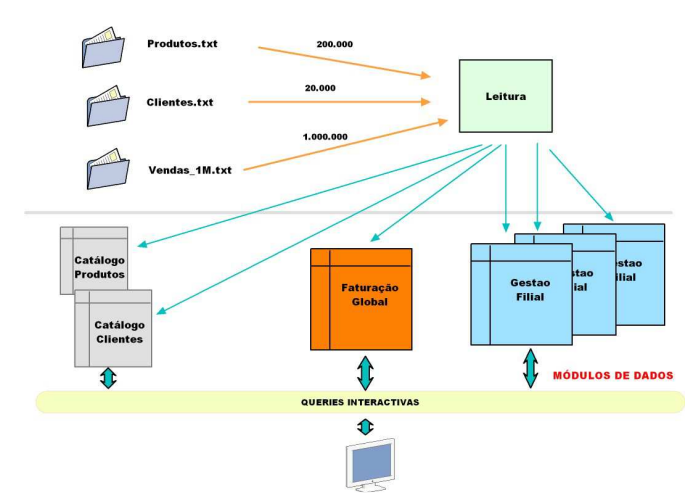
\includegraphics[scale=0.8]{arquiteturaproj.png}  
	\caption{Arquitetura da aplicação}  
\end{figure}


\chapter{Diagrama de classes}
De seguida é apresentado o Diagrama de classes gerado no BlueJ com os ficheiros .java usados. 

\begin{figure}[h!]
	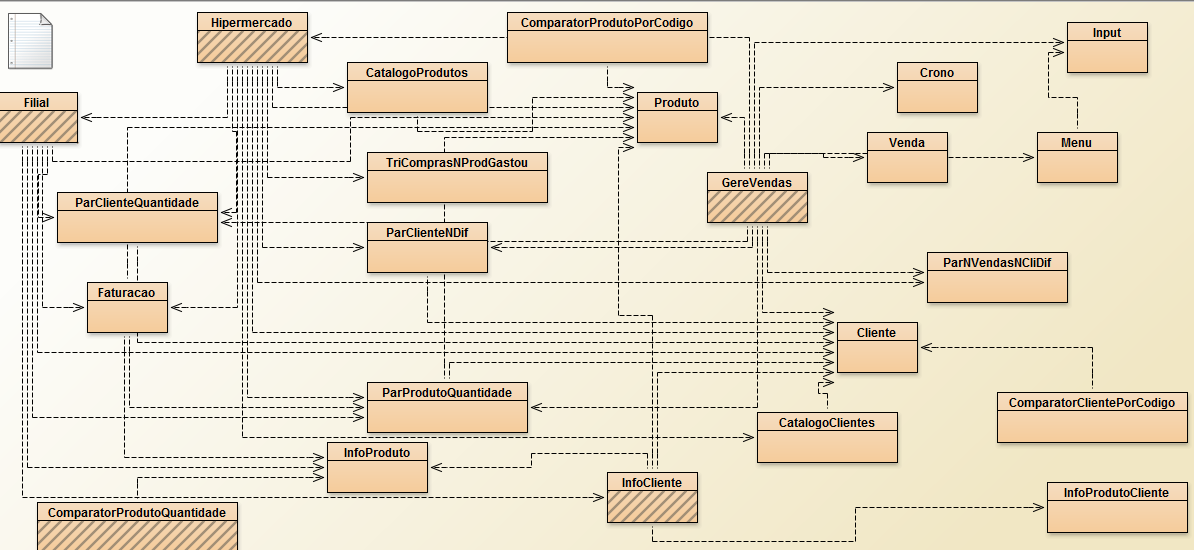
\includegraphics[scale=0.55]{diagramaclasses.png}  
	\caption{Diagrama de classe do Blue J }  
\end{figure}

\chapter{Módulos de dados}

\section{Catálogo de Clientes}
É o módulo de dados onde são guardados os códigos de todos os clientes do ficheiro \textbf{Clientes.txt}, organizados por índice alfabético;

\subsection{Classe CatalogoClientes} 

Para guardar os clientes presentes no ficheiro de clientes, criámos a classe \color{blue} \textbf{CatalogoClientes} \color{black} que
irá guardar clientes e manter a lista dos que não realizaram nenhuma compra.
Para além disso cria a lista com todos os códigos de cliente a partir de uma letra inicial do código. Visto que o catálogo apenas deveria guardar os códigos de clientes decidimos criar a classe \color{blue} \textbf{CatalogoClientes}
\color{black} que guarda todos os códigos de cliente do tipo \color{blue} \textbf{String} \color{black} num HashSet, proporcionando assim uma pesquisa rápida.

\begin{Verbatim}
private Set<Cliente> catalogoClientes;
\end{Verbatim}


\subsection{Classe Cliente}
A classe \color{blue} \textbf{Cliente} \color{black} foi implementada para validar os clientes. Foi utilizada a classe especial em Java que é responsável por fazer comparações de objetos, que é a classe \color{blue} Comparable \color{black}. Usada como padrão de comparação, serve para comparar o tipo de objectos para os quais o objeto  Cliente pode ser comparado. 

 

\begin{Verbatim}
public class Cliente implements Comparable<Cliente> {

	private String codigo_cliente;
\end{Verbatim}



\subsection{Classe InfoCliente}

Fica aqui o código que define as variáveis de instância da classe InfoCliente:

\begin{Verbatim}
class InfoCliente {
private double[] dinheiroGastoMes;
private int[] totalCompradoMes;
private int [] vendas;
private int totalComprado;
private double totalGasto;
private Map <Produto,InfoProdutoCliente> produtosComprados[]; // modos N P

\end{Verbatim}

\begin{verbatim}
TreeMap <>();
\end{verbatim}



Com estas é possivel descrever o comportamento que um cliente tem, por exemplo o dinheiro gasto por mês. 
 e indica se a compra efetuada foi em modo de Promoção(P), ou em modo Normal (N). 


Esta classe contém os construtores, clone e os respetivos set e get definidos que servirão de auxilio noutras classes. 



\section{Catálogo de Produtos}

 Módulo de dados onde são guardados os códigos de todos os produtos do ficheiro \textbf{Produtos.txt}, organizados por índice alfabético, o que irá permitir, de forma eficaz, saber quais são os produtos cujos códigos começam por uma dada letra do alfabeto e saber quantos produtos são contabilizados. 
 
 \subsection{Classe CatalogoProdutos}

\begin{verbatim}
private Set<Produto> catalogoProdutos;
\end{verbatim}

\subsection{Classe InfoProduto}

\begin{verbatim}
public class InfoProduto {
private int [][] quantidade; // [12][3] mes, filial
private int quantidadeTotal;
private double [][] faturado; // [12][3] mes, filial
private double totalFaturado;
private int[][] vendas;
\end{verbatim}



\subsection{Classe Produto}


\begin{verbatim}
public class Produto implements Comparable<Produto> {

private String codigo_produto;
\end{verbatim}




\section{Faturação Global}

Módulo de dados que contém as estruturas de dados responsáveis pela resposta a questões quantitativas que relacionam os produtos às suas vendas mensais, em modo Normal (N) ou em Promoção (P), para cada um dos casos guardando o número de vendas e o valor total de faturação de cada um destes tipos. Este módulo refecencia todos os produtos, mesmo os que nunca foram vendidos, não contém qualquer referência a clientes, mas é capaz de distinguir os valores obtidos em cada filial. 

\begin{verbatim}
public class Faturacao {
private int totalVendas;
private double totalFaturado;
private HashMap<Produto, InfoProduto> produtosVendidos;
\end{verbatim}



\section{Gestão da Filial}

Módulo de dados que, a partir dos ficheiros lidos, contém as estruturas de dados adequadas à representação dos relacionamentos, fundamentais para a aplicação, entre produtos e clientes, ou seja, para cada produto, saber quais os clientes que o compraram, quantas unidades cada um comprou, o mês e a filial.

 Para a estruturação optimizada dos dados deste módulo de dados tivemos em atenção que pretendemos ter o histórico de vendas organizado por filial para uma melhor análise, nunca esquecendo que existem 3 filiais nesta cadeia. 


\begin{verbatim}
public class Filial {
private Map<Cliente,InfoCliente> informacaoClientes; 
\end{verbatim}

\section{Classe Hipermercado }

\begin{verbatim}

public class Hipermercado implements Serializable {

private CatalogoClientes clientes;
private CatalogoProdutos produtos;
private Filial filiais[];
private Faturacao faturacao;
private String ficheiroLido;
private int vendaserradas;
private int totalprodutos;
private int totalclientes;
private int totalcompraram;
private int totalnaocompraram;
private int comprasnulas;
private double faturacaoglobal;
\end{verbatim}

\section{Classes Auxiliares}

\subsection{ParClienteNDif}




\chapter{Interface com utilizador}

Nesta secção apresenta-se a interface com o utilizador, fazendo algumas considerações sobre as decisões tomadas.
Ao iniciar o programa, o utilizador tem um menu que lhe permite escolher 4 opções para ler os ficheiros:




\chapter{Resultados e comentários sobre os testes de performance}

O programa foi corrido num computador blablabla bla com xxxpto. 

Depois de desenvolver e codificar todo o projeto foi-nos proposto realizar alguns testes de performance que consistem em comparar os tempos de execução das queries 8, 9, 10, 11 e 12 usando os ficheiros Vendas\_1M.txt (1 000 000 vendas), Vendas\_3M.txt (3 milhões de vendas) e Vendas\_5M.txt (5 milhões de vendas).


\section{Performance Leitura dos Ficheiros}




\section{Performance Queries }


Foram consideradas 4 situações diferentes, a primeira situação é onde a estrutura do módulo de
compras, a class \color{blue} \textbf{ola} \color{black} tem a sua estrutura definida da seguinte forma:

\begin{verbatim}

\end{verbatim}

\par Na segunda situação a estrutura foi modifica para em vez de utilizar \color{blue} \textbf{TreeMap} \color{black} utilizar um
\color{blue} \textbf{HashMap} \color{black}. Ficando então a estrutura definida da seguinte forma:

\begin{verbatim}

\end{verbatim}

\par Na terceira situação a estrutura foi modifica para em vez de utilizar \color{blue} \textbf{ArrayList} \color{black} utilizar a
classe  \color{blue} \textbf{Vector} \color{black} . Ficando então a estrutura definida da seguinte forma:

\begin{verbatim}

\end{verbatim}

\par A útima situação, situação 4 é a mistura da situação 2 e 3, ficando a estrutura definida da seguinte forma:

\begin{verbatim}

\end{verbatim}

\par Para medir os tempos executamos as queries 5,6,7,8 e 9. Na query 8 utilizamos 1000 produtos como o número base
para os testes e na query 9 utilizamos 1000 clientes. Para a query 10, para cada uma das situações corremos 5 vezes,
para os produtos: "HO2915", "GF7879", "EN3727", "TM3887", "KN1847" e 1000 clientes, no final calculamos a média destas 5
execuções e foi o tempo que registamos.
\par De seguida apresentamos a tabela dos tempos registados seguido de um gráfico que irá ajudar na conclusão destes
testes de performance das diferentes estruturas.


  	